\documentclass{meam520}     
\usepackage[letterpaper,top=0.5in,bottom=0.5in,left=1.2in,right=1.2in,includeheadfoot]{geometry}
\usepackage{amssymb,amsmath}
\usepackage{parskip}
\usepackage{fancyhdr}
\usepackage{tabu}
\usepackage{enumerate}
\usepackage{graphicx}
\usepackage{xcolor}
\usepackage{mathtools}
\usepackage{hyperref}

\hypersetup{
    colorlinks=true,
    linkcolor=blue,
    filecolor=magenta,      
    urlcolor=cyan,
    pdftitle={Sharelatex Example},
    bookmarks=true,
    pdfpagemode=FullScreen,
    }
    
\urlstyle{same}

\DeclarePairedDelimiter\ceil{\lceil}{\rceil}
\DeclarePairedDelimiter\floor{\lfloor}{\rfloor}
\newcommand{\qed}{\hfill $\blacksquare$}      
\newcommand{\vv}{\bigg}      
\newcommand{\multichoose}[2]{\left(\!\genfrac{(}{)}{0pt}{}{#1}{#2}\!\right)}
\renewcommand{\baselinestretch}{1.3}
\pagestyle{fancy}

\renewcommand{\frac}[2]{\dfrac{#1}{#2}}

\hwauthor{Dinesh Jagai}{dinesh97@seas.upenn.edu}
\hwcourse{MEAM 520}
\hwrecitation{}
\hwno{0}
\hwpartner{

}
\date{}  % uncomment this line to suppress the current date in the title
\date{Due: Monday 1st June 2020}  % or uncomment this line to manually add a date
% \hwonelateday                   % uncomment either this line or the next to
% \hwtwolatedays                  % indicate that you are using an extension

\begin{document}
\maketitle

%Problem 1 
\hwproblem
There are $5$ degrees of freedom in the simulation robot disregarding the gripper.  
%Problem 1 
\hwproblem
Without the gripper the simulation robot has a (\textttt{RRRRR}) configuration. \\ 
With the gripper the simulation robot has a (\textttt{RRRRRP}) configuration. 


%Problem 1 
\hwproblem

\renewcommand{\thefigure}{3.1}
\begin{center}
    \begin{figure}[hbt!]
        \centering
        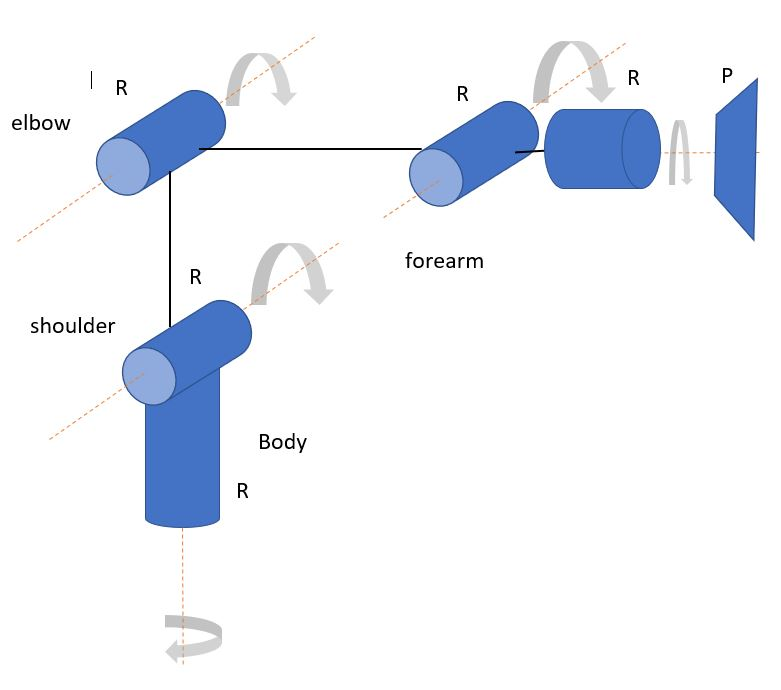
\includegraphics[width=16cm]{P2.JPG}
         \caption{Diagram Showing the 3D symbolic representation of the robot in the zero configuration }
    \end{figure}
\end{center}


%Problem 1 
\hwproblem
\renewcommand{\thefigure}{4.1}
\begin{center}
    \begin{figure}[hbt!]
        \centering
        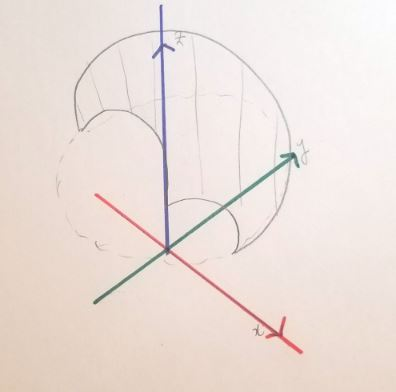
\includegraphics[width=16cm]{p4.JPG}
         \caption{Diagram Showing the h the reachable workspace of the simulated robot }
    \end{figure}
\end{center}

%Problem 1 
\hwproblem
The end effector is pointing \textbf{up}
%Problem 1 
\hwproblem
Joints = $[J_0, J_1, J_2, J_3, J_4, \text{Gripper}]$ \\ 
for $J_0 $ Lower Limit $ = -1.4 $, Upper Limit $ =  1.4 $ \\
for $J_1 $ Lower Limit $ = -1.2 $, Upper Limit $ = 1.4 $ \\
for $J_2 $ Lower Limit $ = -1.8 $, Upper Limit $ =  1.7 $ \\
for $J_3 $ Lower Limit $ =  -1.9 $, Upper   Limit $ = 1.7 $ \\
for $J_4 $ Lower Limit $ =  -2.0 $, Upper Limit $ = 1.5 $ \\
for $\text{Gripper} $ Lower Limit $ =  -15 $, Upper Limit $ = 30 $ \\


%Problem 1 
\hwproblem
Run \texttt{lab0\_v3.py} with $\texttt{q = [0,0,-np.pi/2,-np.pi/2,-np.pi/2,0]}$\\ 
%Problem 1 
\hwproblem
%Problem 1
The stimulation models the movements of the robot for general values of $q$ well. However, for values of $q$ close to the upper an lower limit of each joint, the stimulation sometimes gives erroneous and unrealistic outcomes that actual robot wouldn't stimulate. For example, consider the value of $\texttt{q = [0,0,1.7,1.7,0,0]}$, we have the following configuration as shown in figure 8.1 stimulated by the robot. This can't physically happen with hardware. Furthermore, the movements of the stimulation is fast, at least, faster than the real robot. 
Penultimately, the stimulation doesn't account for the fact that the robot will deteriorate over time. 
Lastly, in the video it seems that certain joints in the robot rotated more than the theoretical limits found on the stimulation. 


\renewcommand{\thefigure}{8.1}
\begin{center}
    \begin{figure}[hbt!]
        \centering
        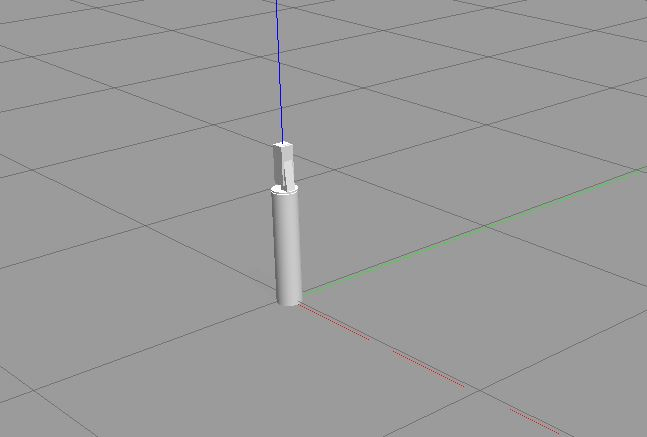
\includegraphics[width=16cm]{p8.JPG}
         \caption{Diagram Showing the 3D symbolic representation of the robot in the for the aforementioned configuration }
    \end{figure}
\end{center}






\end{document}